\section{Global Mincut}

\begin{frame}{Global Mincut History}
    \begin{enumerate}\addtolength{\itemsep}{1em} % Adjust the 1em to increase or decrease space
        \item Recall that a cut means a set of edge $E$ where $G / E$ separate $G$ into two disjoint set $A, B$
        \item Note that \textbf{global mincut} is not the same as $s-t$ mincut aka. max-flow min-cut
        \item \textbf{Global mincut} problem that asks how many edges you have to remove to disconnect a graph
        \item Computing this is hard. The search space is large, exponentially large, however, there is a polynomial time algorithm from Stoer-Wagner computing this in $O(|V||E| + |V|^2\log{|V|})$ time.
        \item Today, let's look at an approximation that runs in $O(|V|^2\text{polylog}{|V|})$ time and returns the minimum cut w.h.p.
    \end{enumerate}
\end{frame}

\begin{frame}[fragile]{Global Mincut Algorithm - Karger}
    \begin{enumerate}
        \item The following subroutine will be useful. The subroutine will keep contracting the graph randomly until there are t vertices left.
        \item It picks an edge described by two vertices on the edge uniformly at random and calls a contract on it.
        \item Contract subroutine is different from what have seen in class. Contract will replace the two vertices, $u, v$, with a new vertex $w$ and take all the adjacent edges of $u, v$ with it. Note that it doesn't merge edges, instead, it keeps all edges so this can be a multigraph.
    \end{enumerate}
    \begin{algorithm}[H]
      \caption{\textsc{Contraction}(Graph G, Integer t) Karger's}
      \begin{algorithmic}
        \While{$|V(G)| > t$}
          \State{$(u, v) \gets$ sample edge $e$ u.a.r from $G$}
          \State{$G \gets$ \textsc{contract}($u, v$)}
        \EndWhile
        \State{return $G$}
      \end{algorithmic}
      \end{algorithm}
\end{frame}

\begin{frame}[fragile]{Global Mincut Algorithm - Karger}
    \begin{figure}
        \centering
        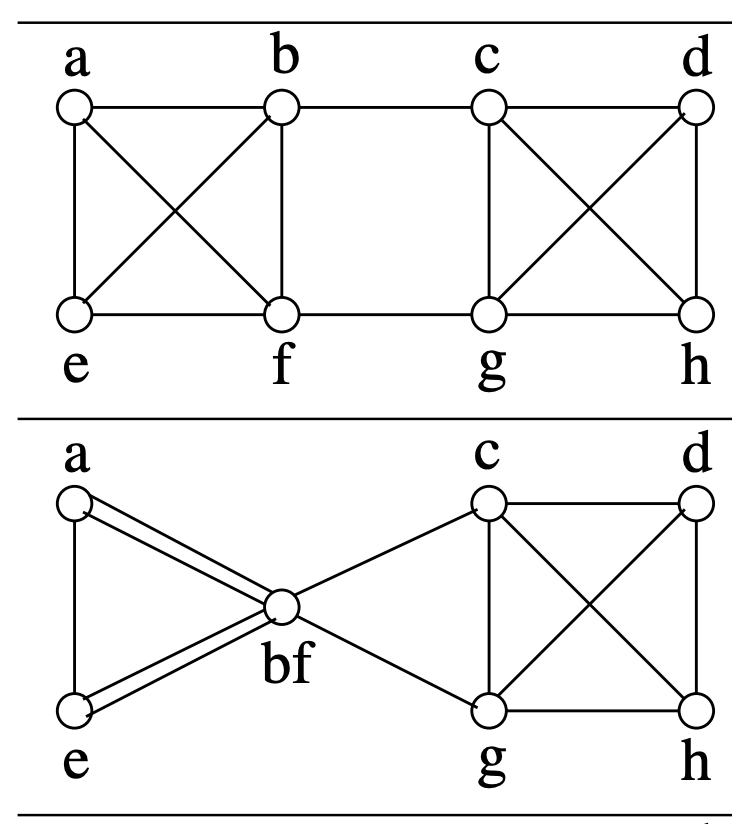
\includegraphics[height=6cm]{images/contraction.png}
        \caption{Contraction example}
        \label{fig:contraction}
    \end{figure}
\end{frame}

\begin{frame}[fragile]{Global Mincut Algorithm}
    \begin{enumerate}
        \item To find mincut, we call contraction(2). This produces a graph with two vertices at the end, therefore we easily get a cut which is the leftover edges between them.
    \end{enumerate}
    \begin{figure}
        \centering
        
\includegraphics[height=1cm]{images/last-iter-contract.png}
        \caption{contraction(2) result. \cite{Arora_2010}}
        \label{fig:contraction-result}
    \end{figure}
\end{frame}

\begin{frame}{Edge Survivability Probability Bound}
    \setlength{\abovedisplayskip}{0pt}
    \setlength{\belowdisplayskip}{0pt}
    \setlength{\abovedisplayshortskip}{0pt}
    \setlength{\belowdisplayshortskip}{0pt}
    \begin{lemma}
        Let contraction($t$) be defined as above, then after $t$ iterations, the probability of min-cut edge surviving is,
        \[\textbf{Pr}[\text{mincut edges survive}] \geq \frac{t(t - 1)}{n(n - 1)} = \Omega\left(\frac{t^2}{n^2}\right)\]
    \end{lemma}
    \begin{lemma}[Edge Survivability Probability Bound]
        \label{edge-surv-prob}
        The probability of min-cut edges being selected for contraction after $i^{th}$ round is,
        \[\textbf{Pr}[\text{min-cut edge selected}] \leq \frac{2}{n - i}\]
    \end{lemma}

\end{frame}

\begin{frame}{Edge Survival Probability After $t$ Iterations}
    \setlength{\abovedisplayskip}{4pt}
    \setlength{\belowdisplayskip}{4pt}
    \setlength{\abovedisplayshortskip}{4pt}
    \setlength{\belowdisplayshortskip}{4pt}
    \begin{proofs}
        \begin{gather*}
            \intertext{We first calculate the probability of a mincut edge being selected. Let $k$ be the minimum edge cut set size, and $i^{th}$ be the iteration, then the probability that we will select any $e_j$ is}
            \textbf{Pr}[Any \text{$e_j$ selected}] = k/|E|\\
            \intertext{Consider the number of edges in the graph. We know that,}
            |E| \geq (n - i)k/2\\
            \intertext{Otherwise, we can produce a smaller min edge cut set. Combining this yields,}
            \textbf{Pr}[\text{$e_j$ selected}] = \frac{k}{|E|} \leq \frac{k}{k(n - i)/2} = \frac{2}{n - i}\\
            \intertext{Therefore, the probability that no $e_j$ is selected is}
            \textbf{Pr}[\text{no $e_j$ selected}] \geq 1 - \frac{2}{n - i}
        \end{gather*}
    \end{proofs}
\end{frame}

\begin{frame}[fragile]{Karger's Analysis}
    \setlength{\abovedisplayskip}{5pt}
    \setlength{\belowdisplayskip}{5pt}
    \setlength{\abovedisplayshortskip}{5pt}
    \setlength{\belowdisplayshortskip}{5pt}
    \begin{proof}
        \begin{align*}
        \intertext{Let the event that after $t$ iterations the mincut edges survive by $E_s$, and $E_i$ be an event that in the iteration $i^{th}$, the edges survive. Then, by the above inequality}
        \textbf{Pr}[E_s] &= \prod_{i = 0}^{n - t - 1}\textbf{Pr}[E_i]\geq \prod_{i = 0}^{n - t - 1}\left(1 - \frac{2}{n - i}\right) = \prod_{i = 0}^{n - t - 1}\left(\frac{n - i - 2}{n - i}\right)\\
        &= \frac{n -2}{2} \cdot \frac{n - 3}{n -1} \cdot \frac{n -4}{n - 2} \cdot \hdots \cdot \frac{t + 1}{t + 3} \cdot \frac{t}{t + 2} \cdot \frac{t - 1}{t + 1}\\
        &= \frac{t(t - 1)}{n(n - 1)} = \Omega\left(\frac{t^2}{n^2}\right)
    \end{align*}
    \end{proof}
    If $t = 2$, the probability is $\Omega(1/n^2)$, therefore we should run this $n^2$ times to get the mincut. Contraction runs in $O(n^2)$ so total running time is $O(n^4)$.
\end{frame}

\begin{frame}[fragile]{Fast Mincut \cite{Baswana_Sen}}
    \begin{algorithm}[H]
      \caption{\textsc{FastMincut}(Graph G) Karger-Stein's}
      \begin{algorithmic}
            \If{$|V(G)| \leq 6$}
                \State{$C \gets$ brute force mincut}
                \State{return $|C|$}
            \Else
                \State{$t = \ceil{1 + n \sqrt{2}}$}
                \State{$H_1, H_2 \gets$ \textsc{contraction}($G$, $t$), \textsc{contraction($G$, $t$)}}
                \State{$C_1, C_2 \gets$ \textsc{FastMincut}($H_1$), \textsc{FastMincut}($H_2$)}
                \State{return $\min\{C_1, C_2\}$}
            \EndIf
            
      \end{algorithmic}
      \end{algorithm}
\end{frame}

\begin{frame}{Fast Mincut Running Time}
    \setlength{\abovedisplayskip}{0pt} 
    \setlength{\belowdisplayskip}{5pt}
    \setlength{\abovedisplayshortskip}{0pt}
    \setlength{\belowdisplayshortskip}{5pt}
    \begin{theorem}[Fast Mincut Running Time]
        \label{fast-mincut-running-time}
        (i) Let fast-mincut, contraction be defined as above, and $G$ be any connected graph, then the total running time of fast-mincut on $G$ is
        \[T(n) = O(n^2\log{n})\]
        (ii) Moreover, to produce a minimum cut of $G$, we runs $c\log{n}$ copies leading to
        \[T(n) = O(n^2\log^2{n})\]
        with high probability.
    \end{theorem}
    \begin{theorem}[Minimum Cut Probability]
        \label{minimum-cut-prob}
        Running $c\log{n}$ copies of fast-mincut produces a mincut in at least one of the copies with high probability. 
    \end{theorem}
\end{frame}

\begin{frame}{Fast Mincut Running Time - Proof}
    \setlength{\abovedisplayskip}{2pt}
    \setlength{\belowdisplayskip}{0pt}
    \setlength{\abovedisplayshortskip}{2pt}
    \setlength{\belowdisplayshortskip}{0pt}
    \begin{proof}[Fast Mincut Running Time]
        \begin{align*}
            \intertext{To prove (i), we consider the following recurrence of fast-mincut.}
            T(n) &= 2T(\ceil{1 + n/\sqrt{2}}) + O(n^2) \\
            &\approx 2T(n/\sqrt{2}) + O(n^2)\\
            &= \sum_{i = 1}^{2\log{n}} 2^i \cdot \frac{n^2}{2^i} = \sum_{i = 1}^{2\log{n}} n^2\\
            &= O(n^2\log{n})\\
            \intertext{To prove (ii), we use theorem \ref{minimum-cut-prob}, therefore we run $c\log{n}$ copies, so it follows that}
            T(n) &= O(n^2\log^2{n})\\
            \intertext{And it produces a minimum cut with high probability.}
        \end{align*}
    \end{proof}
\end{frame}

\begin{frame}{Fast Mincut Analysis Intuition}
    \begin{figure}
        \centering
        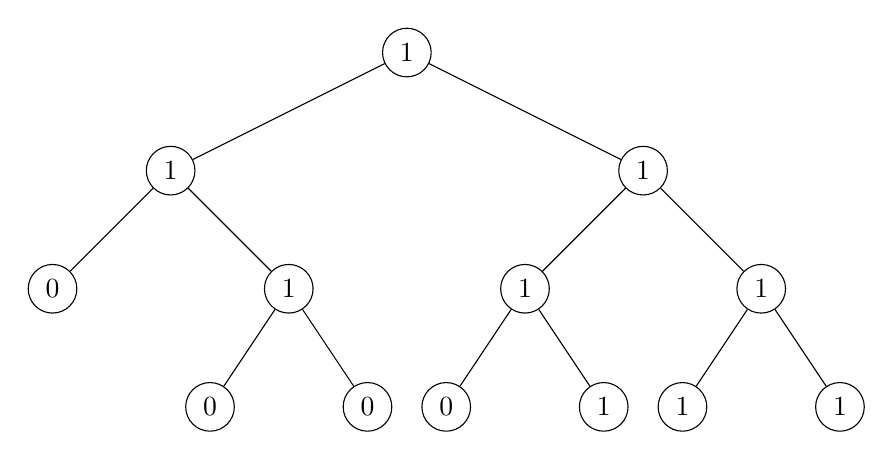
\begin{tikzpicture}[
            level 1/.style={sibling distance=60mm},
            level 2/.style={sibling distance=30mm},
            level 3/.style={sibling distance=20mm},
            level 4/.style={sibling distance=10mm},
        ] % ERROR GONE LET'S FUCKING GOOOOOOOOOOO YAYYYY what the fuck happened
            \node [circle, draw] (root) {1}
            child {
                node [circle, draw] {1}
                child {
                    node [circle, draw] {0}
                    % child {node [circle, draw] {0}}
                    % child {node [circle, draw] {0}}
                }
                child {
                    node [circle, draw] {1}
                    child {node [circle, draw] {0}}
                    child {node [circle, draw] {0}}
                }
            }
            child {
                node [circle, draw] {1}
                child {
                    node [circle, draw] {1}
                    child {node [circle, draw] {0}}
                    child {node [circle, draw] {1}}
                }
                child {
                    node [circle, draw] {1}
                    child {node [circle, draw] {1}}
                    child {node [circle, draw] {1}}
                }
            };
        \end{tikzpicture}
        \caption{Binary Tree representing the process. 1 represents the min-cut still being in the subproblem at recursion depth $l$, and $0$ otherwise.}
        \label{fig:branching-proc}
    \end{figure}
\end{frame}

\begin{frame}{Minimum Cut Probability Proof}
    \begin{enumerate}
        \item To prove theorem \ref{minimum-cut-prob} (minimum cut probability) we need more advanced tools
        \item We here present two proofs one based on \textbf{Stochastic Processes} and sheer power and another we will use Chernoff's bound on offspring distribution
        \item The main idea is to analyze this as a \textbf{Galton-Watson Branching Processes} with approximately binomial offspring distribution
        \item The setup is as follows, for each recursive call of fast-mincut, it produces $H_1$ and $H_2$. If the minimum cut is in $H_i$ we say $Y_i$ produces an offspring. So each $Y_i$ can produce $0, 1,$ or $2$ offspring(s). If $Y_i = 0$, then both $H_1$ and $H_2$ do not contain minimum cut, if $Y_i = 1$ then either one of them contains the cut, and if $Y_i = 2$ both of them contain a cut.
        \item The quantity of interest is then the \textbf{survival probability} after $2\log{n}$ generations. Or simply, $1 - \rho_n$, where $\rho_n$ is the \textbf{probability of extinction} on generation $n$.
    \end{enumerate}
\end{frame}

\begin{frame}{Stochastic Processes - Branching Processes}
    \begin{definition}[Branching Processes]
        A \textbf{Galton-Watson Branching Processes} is a \textbf{Discrete Time Homogenous Markov Chain} that satisfies the following properties. Let $Z_t$ be a random variable counting the number of individuals in generation $t^{th}$ and $Y_i^t$ be individual $i^{th}$ at time $t$. 
        \begin{enumerate}
            \item A population starts with one individual at time $t = 0$ so $Z_0 = 1$.
            \item Every individual lives on a unit of time and produces $Y$ offspring.
            \item $Y$ can tales values $0, 1, 2, \hdots$ with probability $\textbf{Pr}[Y = k]$.
            \item All individuals reproduce independently.
        \end{enumerate}
        The collection of $Z_n = \lbrace Z_0, Z_1, Z_2, \hdots \rbrace, n \in \mathbb{N}$ is called a branching process.
    \end{definition}
\end{frame}

\begin{frame}{Stochastic Processes - Main Theorems}
    \begin{theorem}[Distribution at time $n$]
        Let $G(s) = \mathbb{E}[s^Y] = \sum_{y = 0}^\infty \textbf{Pr}[y = 1]s^y$ be the \textbf{probability generating function} of each individual $Y$. Let $Z_0 = 1$, and $Z_n$ be the population size at time $n$. We now define $G_(s)$ to be the probability generating function of $Z_n$, then
        \[G_n(s) = G\left(G\left(G\left(\hdots G\left(s\right)\hdots\right)\right)\right)\]
        is the composition of $G$ $n$ times.
    \end{theorem}
    \begin{theorem}[Expected Population Size At Time $n$]
        Let $\lbrace Z_0, Z_1, Z_2, \hdots\rbrace$ be a branching process with $Z_0 = 1$. Let $Y$ denote the family size distribution, and suppose that $\mathbb{E}[Y] = \mu$. Then,
        \[\mathbb{E}[Z_n] = \mu^n\]
    \end{theorem}
\end{frame}

\begin{frame}{Stochastic Processes - Main Theorems}
    \begin{theorem}[Extinction Probability]
        Let the branching process be defined as above, $G(s)$ be the generating function of $Y$, $G_n$ be the generating function of $Z_n$, and $\rho_n$ be the extinction probability at generation $n$. Then,
        \[\rho_n = G(\rho_{n - 1}) = G_n(0)\]
        Moreover, 
        \[\rho^* \Longleftrightarrow s = G(s)\]
        where $\rho^* = \lim_{n \to \infty} \rho_n$.
    \end{theorem}
\end{frame}

\begin{frame}{Minimum Cut Probability Proof}
    \setlength{\abovedisplayskip}{2pt}
    \setlength{\belowdisplayskip}{2pt}
    \setlength{\abovedisplayshortskip}{2pt}
    \setlength{\belowdisplayshortskip}{2pt}
    \begin{proofs}[Minimum Cut Probability - Stochastic Processes]
        \begin{gather*}
        \intertext{Let $E$ be the event where mincut edges survive. Then, using t, for finite $n$, we can show that the probability that edge in min-cut will survive contraction(t) is,}
        \textbf{Pr}[E] \geq \frac{t(t - 1)}{n(n - 1)} = \frac{(\ceil{1 + n/\sqrt{2}})(\ceil{1 + n/\sqrt{2}} - 1)}{n(n - 1)} = \frac{n + \sqrt{2}}{2n - 2} > \frac{1}{2}
        \intertext{Since we call this recursively and independent of each other, we can view this as a \textbf{branching process}  where any node can have zero, one or two children depending on if the mincut survived in zero, one or both children. Let $Y_i$ denotes the number of children that individual $Y_i$ has, then}
        \mu = \mathbb{E}[Y_i] = np > 2 \cdot \frac{1}{2} = 1
    \end{gather*}
    \end{proofs}
\end{frame}

\begin{frame}{Fast Mincut Probabilistic Analysis - Stochastic Processes}
    \setlength{\abovedisplayskip}{2pt}
    \setlength{\belowdisplayskip}{2pt}
    \setlength{\abovedisplayshortskip}{2pt}
    \setlength{\belowdisplayshortskip}{2pt}
    \begin{proofs}[Minimum Cut Probability - Stochastic Processes]
        \begin{align*}
            \intertext{Recall from \textbf{Stochastic Processes} the probability that a branching process will be extinct by generation $n$ is $\rho_n = G(\rho_{n - 1}) = G_n(0)$ where $G(\cdot)$ is probability generating function of $Y$, and $G_n(\cdot)$ is $n^{th}$ composition of $G$. Then, taking $p = 1/2$, the lower bound, }
            G(s) &= \sum_{i = 0}^\infty \textbf{Pr}[Y = i]s^i = \frac{1}{4} + \frac{1}{2}s + \frac{1}{4}s^2 = \frac{1}{4}(1 + s)^2\\
            \intertext{Then, for $\rho_n$}
            \rho_n &= \frac{1}{4}(1 + \rho_{n - 1})^2
            \intertext{Now we just need to solve this recurrence.}
        \end{align*}
    \end{proofs}
\end{frame}

\begin{frame}{Recurrence - Oh no...}
    \begin{figure}
        \centering
        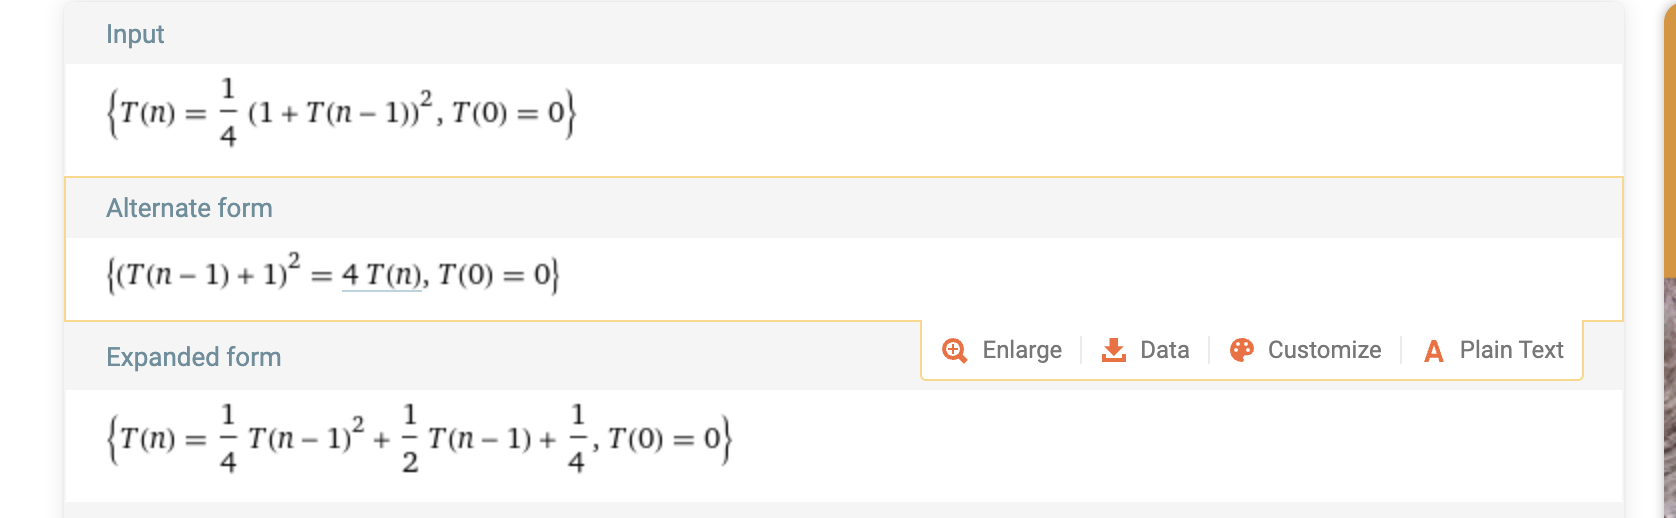
\includegraphics[height=5.5cm]{images/wolfram.png}
        \caption{Wolfram cannot solve this. GG}
    \end{figure}
\end{frame}

\begin{frame}{Recurrence - But Wait.}
    \begin{figure}
        \centering
        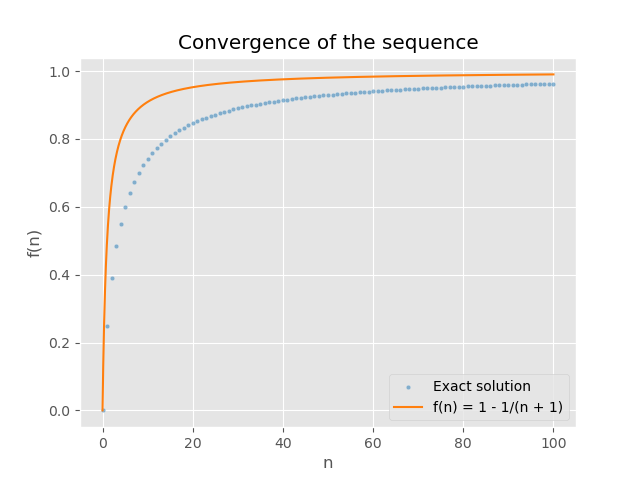
\includegraphics[height=6cm]{images/convergence.png}
        \caption{Asymptotic Recurrence Solution}
    \end{figure}
\end{frame}

\begin{frame}{Fast Mincut Probabilistic Analysis - Stochastic Processes}
    \setlength{\abovedisplayskip}{0pt}
    \setlength{\belowdisplayskip}{0pt}
    \setlength{\abovedisplayshortskip}{0pt}
    \setlength{\belowdisplayshortskip}{0pt}
    \begin{proofs}[Minimum Cut Probability - Stochastic Processes]
        \begin{align*}
            \intertext{With divine intervention (linear regression on sampled points), we claim $\rho_n = O(1 - 1/n)$, then we perform inductive verification. Let $\rho_0 = 0$ and $c = 1$, then}
            \rho_n &= \frac{1}{4}\left(1 + \rho_{n - 1}\right)^2 \leq \frac{1}{4}\left(1 + c - \frac{c}{n - 1}\right)^2 = \frac{\left(n-1+nc-2c\right)^2}{4\left(n-1\right)^2} \leq  \frac{\left(2n-3\right)^2}{4\left(n-1\right)^2}\\
            &= \left(\frac{2n-3}{2n-2}\right)^2 = \left(1 - \frac{1}{2n-2}\right)^2 = 1^2 - 2 \cdot \frac{1}{2n-2}+\left(\frac{1}{2n-2}\right)^2\\
            &= 1 - \frac{1}{n-1} + \frac{1}{(2n-2)^2}\\
            &\leq 1 - \frac{1}{n}\\
            \intertext{For $n \geq 2$. So, the recurrence has asymptotic solution of $O(1 - 1/n)$}
        \end{align*}
    \end{proofs}
\end{frame}

\begin{frame}{Fast Mincut Probabilistic Analysis - Stochastic Processes}
    \setlength{\abovedisplayskip}{2pt}
    \setlength{\belowdisplayskip}{2pt}
    \setlength{\abovedisplayshortskip}{2pt}
    \setlength{\belowdisplayshortskip}{2pt}
    \begin{proof}[Minimum Cut Probability - Stochastic Processes]
        \begin{gather*}
            \intertext{Since we only consider up to $2\log{n}$ layers, it follows that}
            \rho_n = 1 - 1/n = 1 - 1/\log{n} \leq \exp\left\{-1/\log{n}\right\}
            \intertext{Then, if we repeat this $c\log^2{n}$ times, we get that}
            \rho_n = \prod_{i = 0}^{c\log^2{n}}\exp\left\{-1/\log{n}\right\} = \exp\left\{-c\frac{\log^2{n}}{\log{n}}\right\} = \exp\left\{\log{n^{-c}}\right\} = \frac{1}{n^c}
            \intertext{So the probability of survival after $c\log^2{n}$ runs is,}
            \textbf{Pr}[\text{mincut edge survive}] \geq 1 - \frac{1}{n^c}
            \intertext{which occurs with high probability.}
        \end{gather*}
    \end{proof}
\end{frame}

\begin{frame}{Fast Mincut Probabilistic Analysis - Chernoff}
    \setlength{\abovedisplayskip}{5pt}
    \setlength{\belowdisplayskip}{5pt}
    \setlength{\abovedisplayshortskip}{5pt}
    \setlength{\belowdisplayshortskip}{5pt}
    \begin{proofs}[Minimum Cut Probability - Chernoff]
        \begin{align*}
            \intertext{Here, we also show Chernoff-based proof. Consider the number of individuals on generation $n$. Let,}
            X_i &= \begin{cases}
                1, \text{if the individual is present},\\
                0, \text{otherwise, i.e parent doesn't reproduce}
            \end{cases}\\
            \intertext{and,}
            X &= \sum_i X_i\\
            \intertext{Consider the quantity $\mathbb{E}[X]$ which is the expected number of individual in generation $n$. We know that this is the same as}
            \mathbb{E}[X] &= \mathbb{E}[Z_{n - 1}] = \mu^{n - 1} = (np)^{n - 1} > (1/2 \cdot 2)^{n - 1} = 1
        \end{align*}
    \end{proofs}
\end{frame}

\begin{frame}{Fast Mincut Probabilistic Analysis - Chernoff}
    \setlength{\abovedisplayskip}{0pt}
    \setlength{\belowdisplayskip}{0pt}
    \setlength{\abovedisplayshortskip}{0pt}
    \setlength{\belowdisplayshortskip}{0pt}
    \begin{proof}[Minimum Cut Probability - Chernoff]
        \begin{align*}
            \intertext{Since each $X_i \sim I(p)$ and $i.i.d$, for $\delta = 1/2$, using Chernoff's we obtain,}
            \textbf{Pr}[X \leq (1 - \delta)\mathbb{E}[X]] &= \textbf{Pr}[X \leq (1 - \delta)\mathbb{E}[Z_n]] \leq \exp\left\{- \frac{\delta^2}{2}\mu^{n - 1}\right\} \leq \exp\left\{- \frac{1}{8}\right\}\\
            \intertext{If we run the algorithm $c\log{n}$ times, the probability of failure is at most}
            \textbf{Pr}[\text{fail}] &\leq (\exp\{-1/8\})^{c\log{n}} = \exp\left\{\log{n^\frac{-c}{8}}\right\} = \frac{1}{n^{c/8}}
            \intertext{So, the probability of at least one success after $c\log{n}$ is}
            \textbf{Pr}[\text{survive}] &\geq \textbf{Pr}[X \leq (1 - \delta)\mathbb{E}[X]] = \textbf{Pr}[X > 1/2] = \textbf{Pr}[X \geq 1/2]\\ &= 1 - \frac{1}{n^{c/8}} = 1 - \frac{1}{n^c} = 1 - O\left(\frac{1}{n}\right)
            \intertext{which occurs with high probability.}
        \end{align*}
    \end{proof}
\end{frame}



